\documentclass[tikz,border=4pt]{standalone}
\usetikzlibrary{arrows.meta,calc,positioning}
\begin{document}
\pagecolor{white}
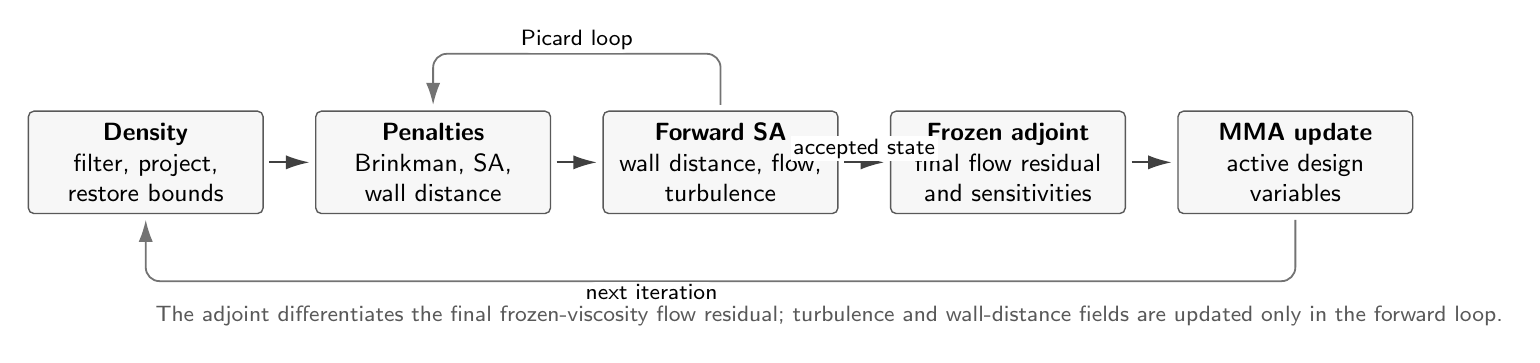
\begin{tikzpicture}[
  font=\sffamily\small,
  stage/.style={
    draw=black!65,
    rounded corners=2pt,
    line width=0.5pt,
    align=center,
    minimum height=13mm,
    text width=27mm,
    inner xsep=4pt,
    inner ysep=3pt,
    fill=black!3
  },
  arrow/.style={-{Latex[length=3mm,width=1.8mm]}, line width=0.7pt, draw=black!75, shorten <=2pt, shorten >=2pt},
  loop/.style={-{Latex[length=2.8mm,width=1.8mm]}, line width=0.65pt, draw=black!55, rounded corners=5pt, shorten <=2pt, shorten >=2pt}
]

\node[stage] (density) at (0,0) {\textbf{Density}\\filter, project,\\restore bounds};
\node[stage] (physics) at (3.65,0) {\textbf{Penalties}\\Brinkman, SA,\\wall distance};
\node[stage] (forward) at (7.30,0) {\textbf{Forward SA}\\wall distance, flow,\\turbulence};
\node[stage] (adjoint) at (10.95,0) {\textbf{Frozen adjoint}\\final flow residual\\and sensitivities};
\node[stage] (mma) at (14.60,0) {\textbf{MMA update}\\active design\\variables};

\draw[arrow] (density) -- (physics);
\draw[arrow] (physics) -- (forward);
\draw[arrow] (forward) -- node[above, fill=white, inner sep=1pt, font=\sffamily\footnotesize]
  {accepted state} (adjoint);
\draw[arrow] (adjoint) -- (mma);

\draw[loop] (mma.south) -- ++(0,-0.85) -| node[pos=0.28, below, fill=white, inner sep=1pt, font=\sffamily\footnotesize]
  {next iteration} (density.south);

\draw[loop] (forward.north) -- ++(0,0.72) -| node[pos=0.25, above, fill=white, inner sep=1pt, font=\sffamily\footnotesize]
  {Picard loop} (physics.north);

\node[anchor=west, font=\sffamily\footnotesize, text=black!65] at (0,-1.95)
  {The adjoint differentiates the final frozen-viscosity flow residual; turbulence and wall-distance fields are updated only in the forward loop.};

\end{tikzpicture}
\end{document}
